\documentclass[12pt]{article}
\usepackage[latin2]{inputenc}
\usepackage{t1enc}
\usepackage{amsmath}
\usepackage[magyar]{babel}
\usepackage{graphics}

\usepackage{fullpage}

\usepackage{float} %H-hoz
\usepackage{verbatim}

% \H{o} \H{o}
% \H{u} \H{u}
%


\title{Biztonságkritikus robotrepül\H{o}gép földi állomásának kialakítása\\{\normalsize Önálló laboratórium zárójegyz\H{o}könyv\\2012/13 II. félév}
}
\\
\author{Böjti Paszkál(BH0R0N)\\III. évf, mérnök informatikus szakos hallgató\\
BSc Beágyazott információs rendszerek szakirány
 \\ \\ \\ \\ \\ \\ \\ \\ Konzulens\\Bartha Tamás} 


\begin{document}

\maketitle

\tableofcontents


\section{Motiváció}

Félév során lehet\H{o}ségem volt a SZTAKI Irányítástechnikai Kutató Laboratóriumában egy UAV légi járm\H{u} fejlesztésében részt venni. Az itt kidolgozott szabályozó algoritmusok gyakorlatba való átültetésére egy pilóta nélküli járm\H{u}vet hoztak létre, mely a biztonságos üzemeltetés miatt, illetve az estelegesen el\H{o}fordulható hibák ellen redundáns hardware elemekkel védekezik.
A feladatom e repül\H{o} a földi állomásának a kialakítása volt, mely a redundánsan küldött rádiójelek feldolgozására és megfelel\H{o} megjelenítésre használandó. Az összehasonlításból kiderül, eddig a földi állomásokra nem volt jellemz\H{o} a redundancia. Kutatómunkám során összegy\H{u}jtöttem az UAV-k fejl\H{o}désének történetét, a piacon elérhet\H{o} programokat, összehasonlítottam a megoldásokat, majd ezekb\H{o}l ötletet merítve elkezdtem a program megírását. Konzultációk során finomhangolásokkal a megrendel\H{o} igényeihez formáltam az elképzelt megvalósítást.



\section{Bevezetés}

Napjainkban egyre nagyobb teret hódít a pilóta nélküli légi járm\H{u}vek alkalmazása.
Az 1960-as években a hadszíntéren jelentek meg el\H{o}ször, ahol megfigyelésre, felderítésre, olyan feladatokra használták, ahol kockázatos lett volna emberi életet veszélyeztetni.
Az utóbbi években praktikussága, alacsony üzemeltetési költségei miatt más területeken is hasznosnak bizonyult ez a technológia, pl. geológia mintázatok kutatása, mely az emberi perspektívából nehezen észlelhet\H{o}, t\H{u}zoltósági alakulatok koordinálása, otthoni hobby felhasználás. 



\section{UAV}
\cite{bib:uav}A pilóta nélküli légi járm\H{u} gondolata egészen a XX. század elejére nyúlik vissza, mikor az I. világháborúban egy olyan távirányítású repül\H{o}t alkottak, mely robbanószerrel a fedélzeten a célpontba csapódva okozott kárt.
\cite{bib:sperry}Els\H{o} nagyobb amerikai UAV projekt 1959-ben kezd\H{o}dött, mikor aggódtak az ellenséges területre berepül\H{o} pilóták életéért. Kés\H{o}bb a vietnámi háborúban több mint 3000 küldetésben vett részt ilyen repül\H{o} és mindössze 554 veszett oda. A technológiai korlátok miatt a f\H{o} funkcionalitása video felvétel készítése egy meghatározott útvonalon (általában egyenes vonal, körökkel kiegészítve) repülve, majd a bázisra való visszaérkezés. 
A rádiótechnika fejl\H{o}dése miatt egyre összetettebb feladatok elvégzésére lettek képesek. A nagyobb átviteli sebességnek köszönhet\H{o}en valós id\H{o}ben, monitoron keresztül kezelheti az operátor a távirányítású repül\H{o}t. A mai UAV-k több üzemmódot is támogatnak, egyik az el\H{o}bb említett távirányítás, másik a fedélzeti intelligenciára hagyatkozó. Mind a hagyományos repül\H{o}iparban, mind ebben az érában, szükséges és célszer\H{u} az emberi terhelés csökkentése, utasszállító gépek esetében is a robotpilóta elvégez minden olyan korrekciót, melyet azel\H{o}tt a pilóta folyamatos figyelésével, koncentrációjával lehetett elérni. A modern integrációnak köszönhet\H{o}en, olyan fejlett feldolgozóegységgel dolgozhatjuk fel az adatokat, melyeknek nem jelent\H{o}s a fogyasztása, nem foglalnak sok helyet. A szenzorokból érkez\H{o} információkra, az algoritmusoknak köszönhet\H{o}en úgy tud reagálni, hogy az nem veszélyezteti a repül\H{o} leveg\H{o}ben maradását. Ám hiába a fejlett hardware, a valóban automatikus üzemeltetés még mindig távoli cél, emberi beavatkozás mindig is kelleni fog le,- felszállásoknál, illetve olyan helyzetekben melyre nincs el\H{o}re felkészítve az intelligenciája.


\subsection{UCAV}
\cite{bib:ucav}Katonai felhasználásban elengedhetetlen a fedélzeti fegyverzet, így ezekre a járm\H{u}vekre is felszerelésre került. Az ilyen drónok az estek többségében operátori irányítás alatt állnak, így emberi felel\H{o}sség van a fegyver használata során.

\subsection{Csoportosítás}

Amerikai légier\H{o} ezeket a csoportokat tartja nyilván
\begin{itemize}
\item Kézi indítású: 600 m magasság, 2 km hatótávolság
\item Közeli: 1500 m magasság, 10 km hatótávolság
\item MALE(Medium Altitude,Long Endurance)9 km magasság, 200 km hatótávolság
\item HALE(High Altitude,Long Endurance) 9+ km magasság, 200+ km hatótávolság


\subsection{Felhasználási területek}

\begin{description}
\item[Célpont] kiképzésre használandó, légi fenyegetésként ellenséges célpont
\item[Felderít\H{o}] harctéren nagyobb látóteret biztosít
\item[Támadó] fegyverzettel ellátott, lég-föld, lég-lég rakétákkal csapások mérése
\item[Szállító] raktérrel ellátott, nehezen megközelíthet\H{o} csapatok segítésére
\item[Kísérleti] kés\H{o}bbi UAV-k kifejlesztéséhez
\item[Civil] hétköznapi embereknek szórakozás céljából


\item[Érzékelés] különböz\H{o} érzékel\H{o}kkel ellátva képes kémiai anyagok jelenlétét érzékelni, infrakamerákkal és radarral éjjel is látható az operátor számára a környezet

\item[Megfigyelés] egyik legolcsóbb megfigyelési mód az UAV alkalmazása, kisebb üzemben tartási költsége van, mint egy repül\H{o}nek, pilóta bérének. Pl. vadak vonulásának követése

\item[Geológiai felfedezés] mágneses érzékel\H{o}kkel a Föld mágnesesség változásának mérésével következtetni lehet a föld alatt található ércekre.

\item[Mentés] természeti katasztrófa következtében bajbajutottak segítésére, ment\H{o}csapatok megfelel\H{o} irányba küldésére használatos

\item[Erd\H{o}t\H{u}z detektálás] folyamatosan a megfigyelt terület felett repülve, infravörös kamerával a legkisebb t\H{u}z érzékelhet\H{o}. Szél és egyéb meteorológiai adatokkal szolgáltatva a t\H{u}zoltók munkáját segíti

\end{description}

\subsection{Hosszú repülés}
Mivel az UAV-k nem rendelkeznek fedélzeti személyzettel, így a leveg\H{o}ben töltött idejüket kizárólag az energiaforrásuk sz\H{u}kössége határozza meg. Elektromos meghajtású gépek esetén, megfelel\H{o} méret\H{u} napelem alkalmazása esetén akár végtelenségig leveg\H{o}ben maradhatnak. A minél hosszabb fennmaradás el\H{o}nyös lehet taktika bevetések során, ahol megspórolható az oda-visszaút megtételéb\H{o}l származó kiesés. 
Leghosszabb repült id\H{o} 2010. július. 9 -- 23 közt QinetiQ Zephyr Solar Electric érte el 336 óra 22 perccel (2 hét)

\section{Földi állomás\footnote{GC(S):Ground Control System}}
Egy UAV vezetéséhez elengedhetetlen egy bázis, ahonnan a földi személyzet irányítja, monitorozhatja a repülést. Általában több funkciót lát el:
\begin{itemize}
\item Küldetés tervezés: útvonal meghatározása, illetve a célpontok kijelölése
\item Adatok megjelenítése: megfelel\H{o} módon kijelezni a repül\H{o}gép állapotát, esetleges hibáit.
\end{itemize}

\subsection{Hordozható}
Egy egységbe építették az akkumulátort, kijelz\H{o}t, kezel\H{o}szerveket, hordozhatósága miatt ez az elterjedtebb a kézzel indítható UAV-k esetében.

\begin{figure}[H]
	\centering
	\resizebox{8cm}{!}{
		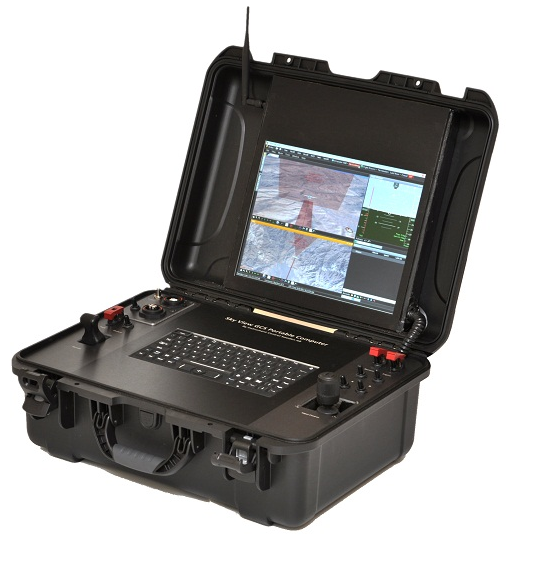
\includegraphics{hord.png}}
	\caption{Hordozható GC}
	\label{fig:hord}
\end{figure}

\subsection{Komplex}
Általában közel a hadszíntérhez üzemeltetik a repül\H{o}ket, így a személyzetet, illetve a felszereléseket páncélozott járm\H{u}vel szállítják, védik.
Pl. az MQ-1 Predator GCS egy utánfutóban helyezkedik el, mely szünetmentes tápegységet biztosít a pilóta és segédszemélyzeti, adatelemz\H{o}/rögzít\H{o} és radar munkaállomásoknak. A kommunikációt UHF és VHF frekvencián bonyolítják közvetlen rálátás esetén, azon kívül m\H{u}hold közbeiktatásával.

\begin{figure}[H]
	\centering
	\resizebox{8cm}{!}{
		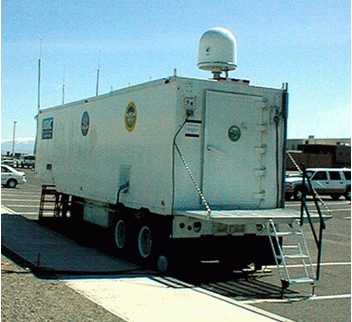
\includegraphics{komplex.png}}
	\caption{Utánfutós megoldás}
	\label{fig:komplex}
\end{figure}


\subsection{Kompatibilitás}
\cite{bib:komp}Ahogy jöttek az újabb gépek, problémát okozott, hogy mindegyik földi állomása különbözött egymástól, így 2008-ban szorgalmaztak egy univerzális GCS architektúrát, mely minden addigi és jöv\H{o}beli katonai UAV-vel ugyanúgy tud kommunikálni, adatokat szolgáltatni. Így született a Raytheon’s Common Ground Control System, melynek fejlesztéséhez videojátékokból merítettek ötleteket. Csökkenteni próbálták a kiképzési id\H{o}t, ne kelljen több hónapos kurzusokon részt venni, hanem úgy, mint egy videojátéknál, kisebb gyakorlás után már tudja az ember, mit hol kell keresni, illetve úgy érezze, hogy valóban \H{o} vezeti a repül\H{o}t.

\begin{figure}[H]
	\centering
	\resizebox{10cm}{!}{
		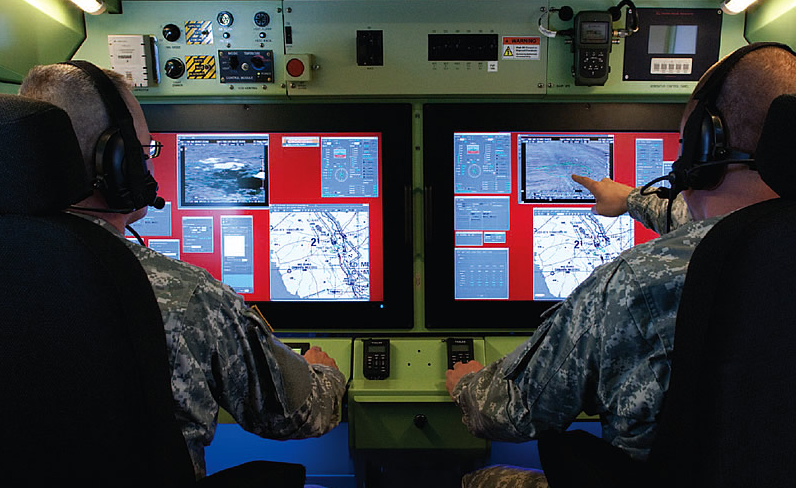
\includegraphics{kompat.png}}
	\caption{UGCS}
	\label{fig:kompat}
\end{figure}


\subsection{Megoldások}
Számos megoldás született a földi állomás GUI\footnote{Graphics User Interface, grafikus megjelenítés}-jának kialakítására. Els\H{o}dleges követelmény, hogy az operátor mindig a legfontosabb információkat láthassa, ehhez szoftverergonómiailag kell megtervezni a m\H{u}szerek, adatok elrendezését.
Az alábbiakban összehasonlításra kerülnek a megjelenítési felületek.

\subsubsection{MIT GCS}
\cite{bib:mit}Els\H{o}dleges megfontolás az volt, hogy a m\H{u}szereket az értékeket linerisan jelenítsék-e meg, mivel az avionikában ez a kérdés már felmerült, így a valós m\H{u}szerek alapján a lineárisat választották. Másodlagos kérdés a m\H{u}szerek formája, itt megvalósítható lenne a csupán digitális értékek kiírása, de szintén a repülésb\H{o}l merítve a kör alakú egységeket választottak

\begin{figure}[H]
	\centering
	\resizebox{10cm}{!}{
		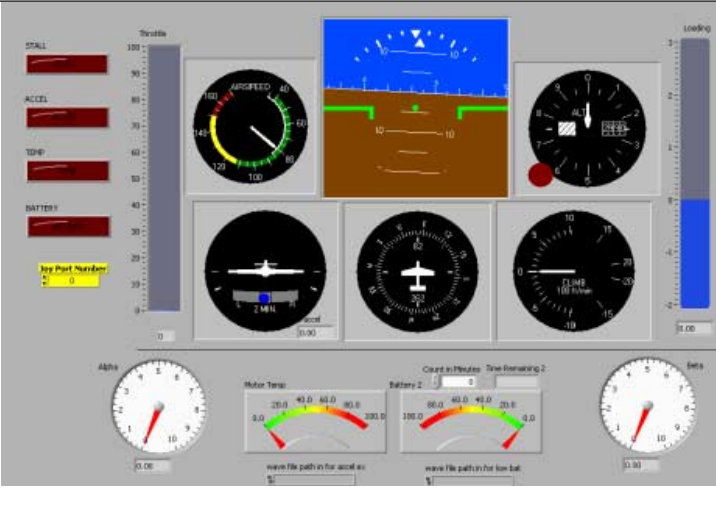
\includegraphics{mit.png}}
	\caption{Alap összeállítás}
	\label{fig:mit}
\end{figure}

\subsubsection{Rodan}
\cite{bib:rodan}Földi, légi, vízi jármüveket is támogat, TCP/IP-n keresztül kommunikál, így videó átküldésére is van sávszélesség. SIL\footnote{Software In the Loop} és HIL\footnote{Hardware In the Loop} támogatás.

A GUI itt már összetettebb, a kamera képe foglalja el a képerny\H{o} nagyobbik részét, mellette egy térképen láthatjuk a járm\H{u} eddigi útvonalát. Egyetlen vizuális m\H{u}szer a m\H{u}horizont, a többi érték csak számadattal van jelezve.

\begin{figure}[H]
	\centering
	\resizebox{10cm}{!}{
		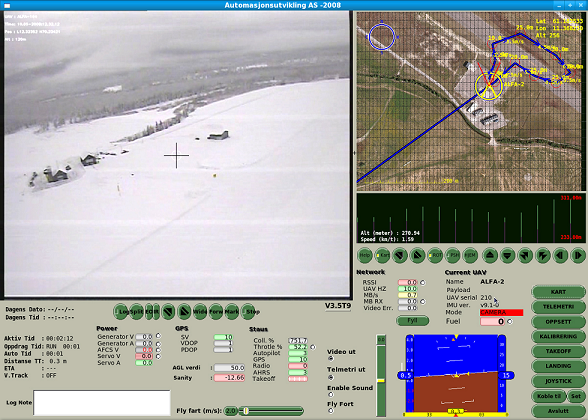
\includegraphics{rodan.png}}
	\caption{Rodan}
	\label{fig:rodan}
\end{figure}

\subsubsection{HappyKillmore}
\cite{bib:hk} Ez a GUI az ArduPlane nev\H{u} nyílt forráskódú, háziépítés\H{u} UAV-hoz készült.
Itt is a térkép nézet dominál, oldalt mozgathatjuk számunkra megfelel\H{o} elrendezésbe a m\H{u}szereket.
Több különböz\H{o} oldal közül választhatunk, ha pl. a bejöv\H{o} adatokra vagyunk kiváncsiak vagy a soros port port számát szeretnénk beállítani. Lehet\H{o}ségünk van exportálni is az adatokat.


\begin{figure}[!h]
	\centering
	\resizebox{10cm}{!}{
		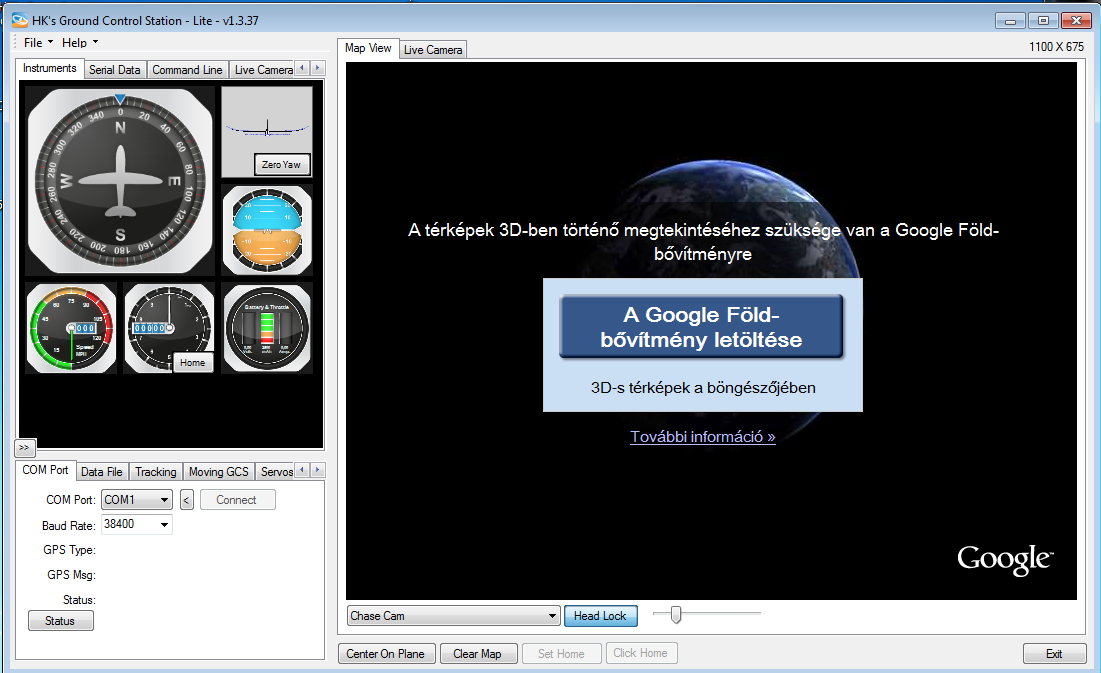
\includegraphics{hk.png}}
		\caption{HK}
	\label{fig:hk}
\end{figure}


\subsubsection{Arducopter}
Az el\H{o}z\H{o}höz hasonlóan ez is az ArduCopterhez készült. Itt lehet\H{o}ségünk van térképen el\H{o}re kijelölni, milyen útvonalat járjon be felszállás után.


\begin{figure}[H]
	\centering
	\resizebox{10cm}{!}{
		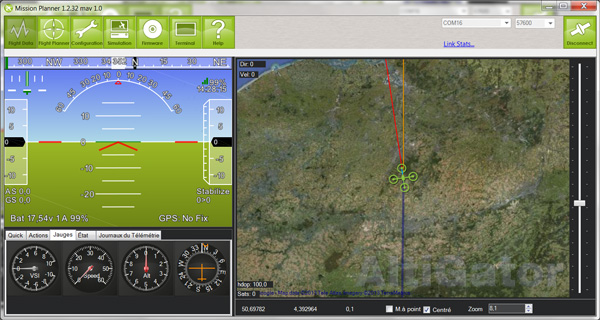
\includegraphics{ardu.png}}
	\caption{Arducopter}
	\label{fig:hk}
\end{figure}


\subsubsection{Viking}
\cite{bib:viking} Itt egyértelm\H{u}en a térkép feletti pozicíón van a hangsúly, jobb oldalt néhány m\H{u}szer, illetve a fontosabb adatok számokkal


\begin{figure}[H]
	\centering
	\resizebox{10cm}{!}{
		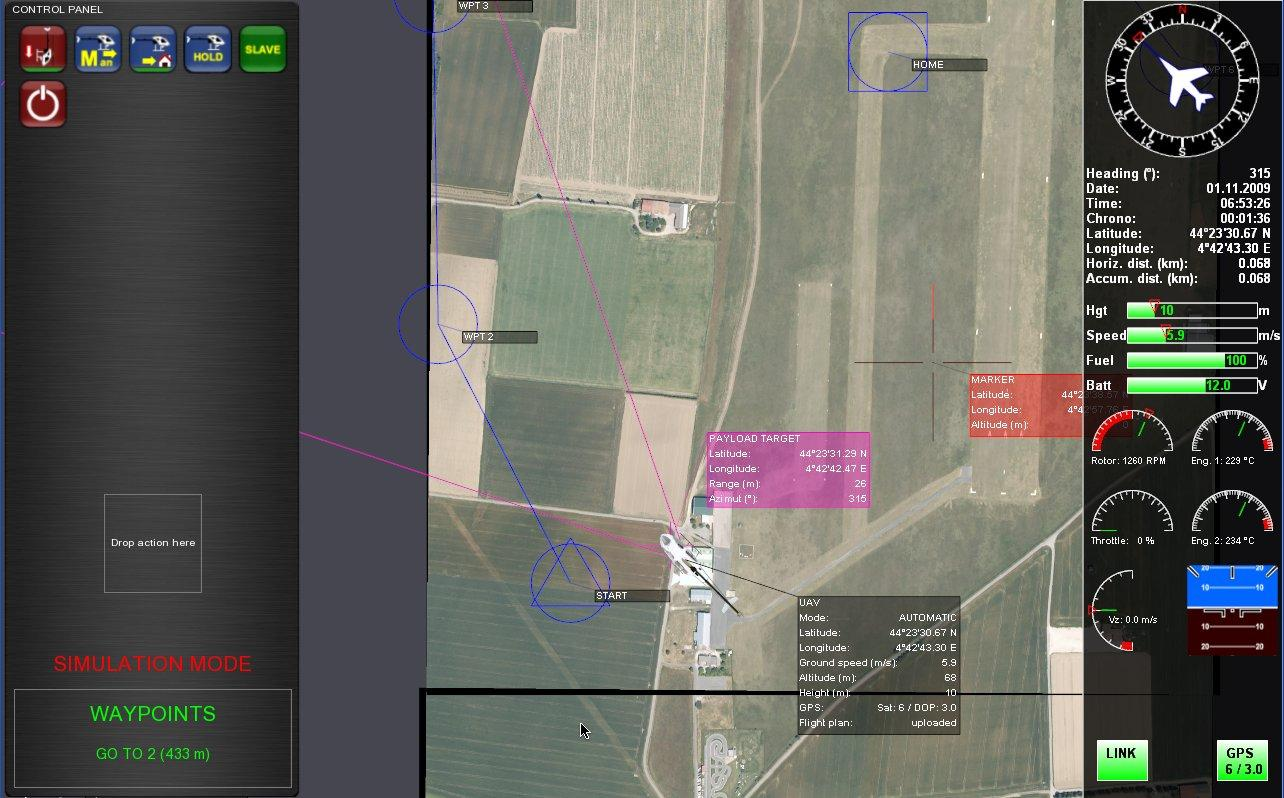
\includegraphics{viking.png}}
	\caption{Viking}
	\label{fig:viking}
\end{figure}







\subsubsection{NI LabWindows™/CVI}
Az el\H{o}z\H{o} Ground control forráskódját átnézve, annak továbbfejlesztése körülményes lenne, így a C\# nyelv  változatos API-jainak köszönhet\H{o}en egy új GUI megírása t\H{u}nik a legoptimálisabb megoldásnak. Soros port kezelésére van beépített \cite{bib:serial}system.io.ports.serialport osztály, mely megkönnyíti az adatok befogadását.




\section{Repül\H{o}gép kialakítása}

A SZTAKI-nak volt már egy hasonló projektje, mely egy kisebb, boltban beszerezhet\H{o} modellrepül\H{o}re épített saját irányítóegységgel repült. A számos tesztnek köszönhet\H{o}en felmerült az igény egy olyan, teljesen saját fejlesztés\H{u} repül\H{o} kialakítására, mely lehet\H{o}séget biztosít biztonságkritikus kialakításra, szemben a gyári alkatrészekkel, amelyek semmilyen visszajelzést nem adnak saját állapotukról, mely a szabályzásban jelent\H{o}s fontossággal bír.

\begin{figure}[H]
	\centering
	\resizebox{10cm}{!}{
		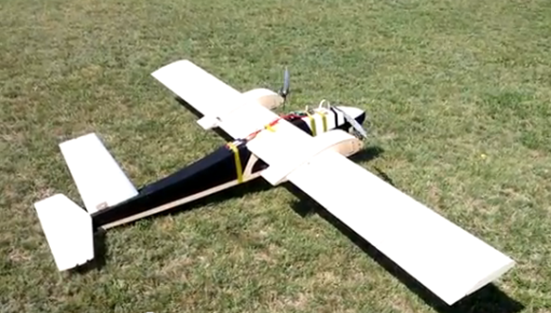
\includegraphics{orca.png}}
	\caption{}
	\label{fig:orca}
\end{figure}

Így az új repül\H{o}gépen redundánsan fog szerepelni:
\begin{itemize}
\item motor
\item akkumulátor
\item központi számítógép
\end{itemize}


\begin{figure}[H]
	\centering
	\resizebox{10cm}{!}{
		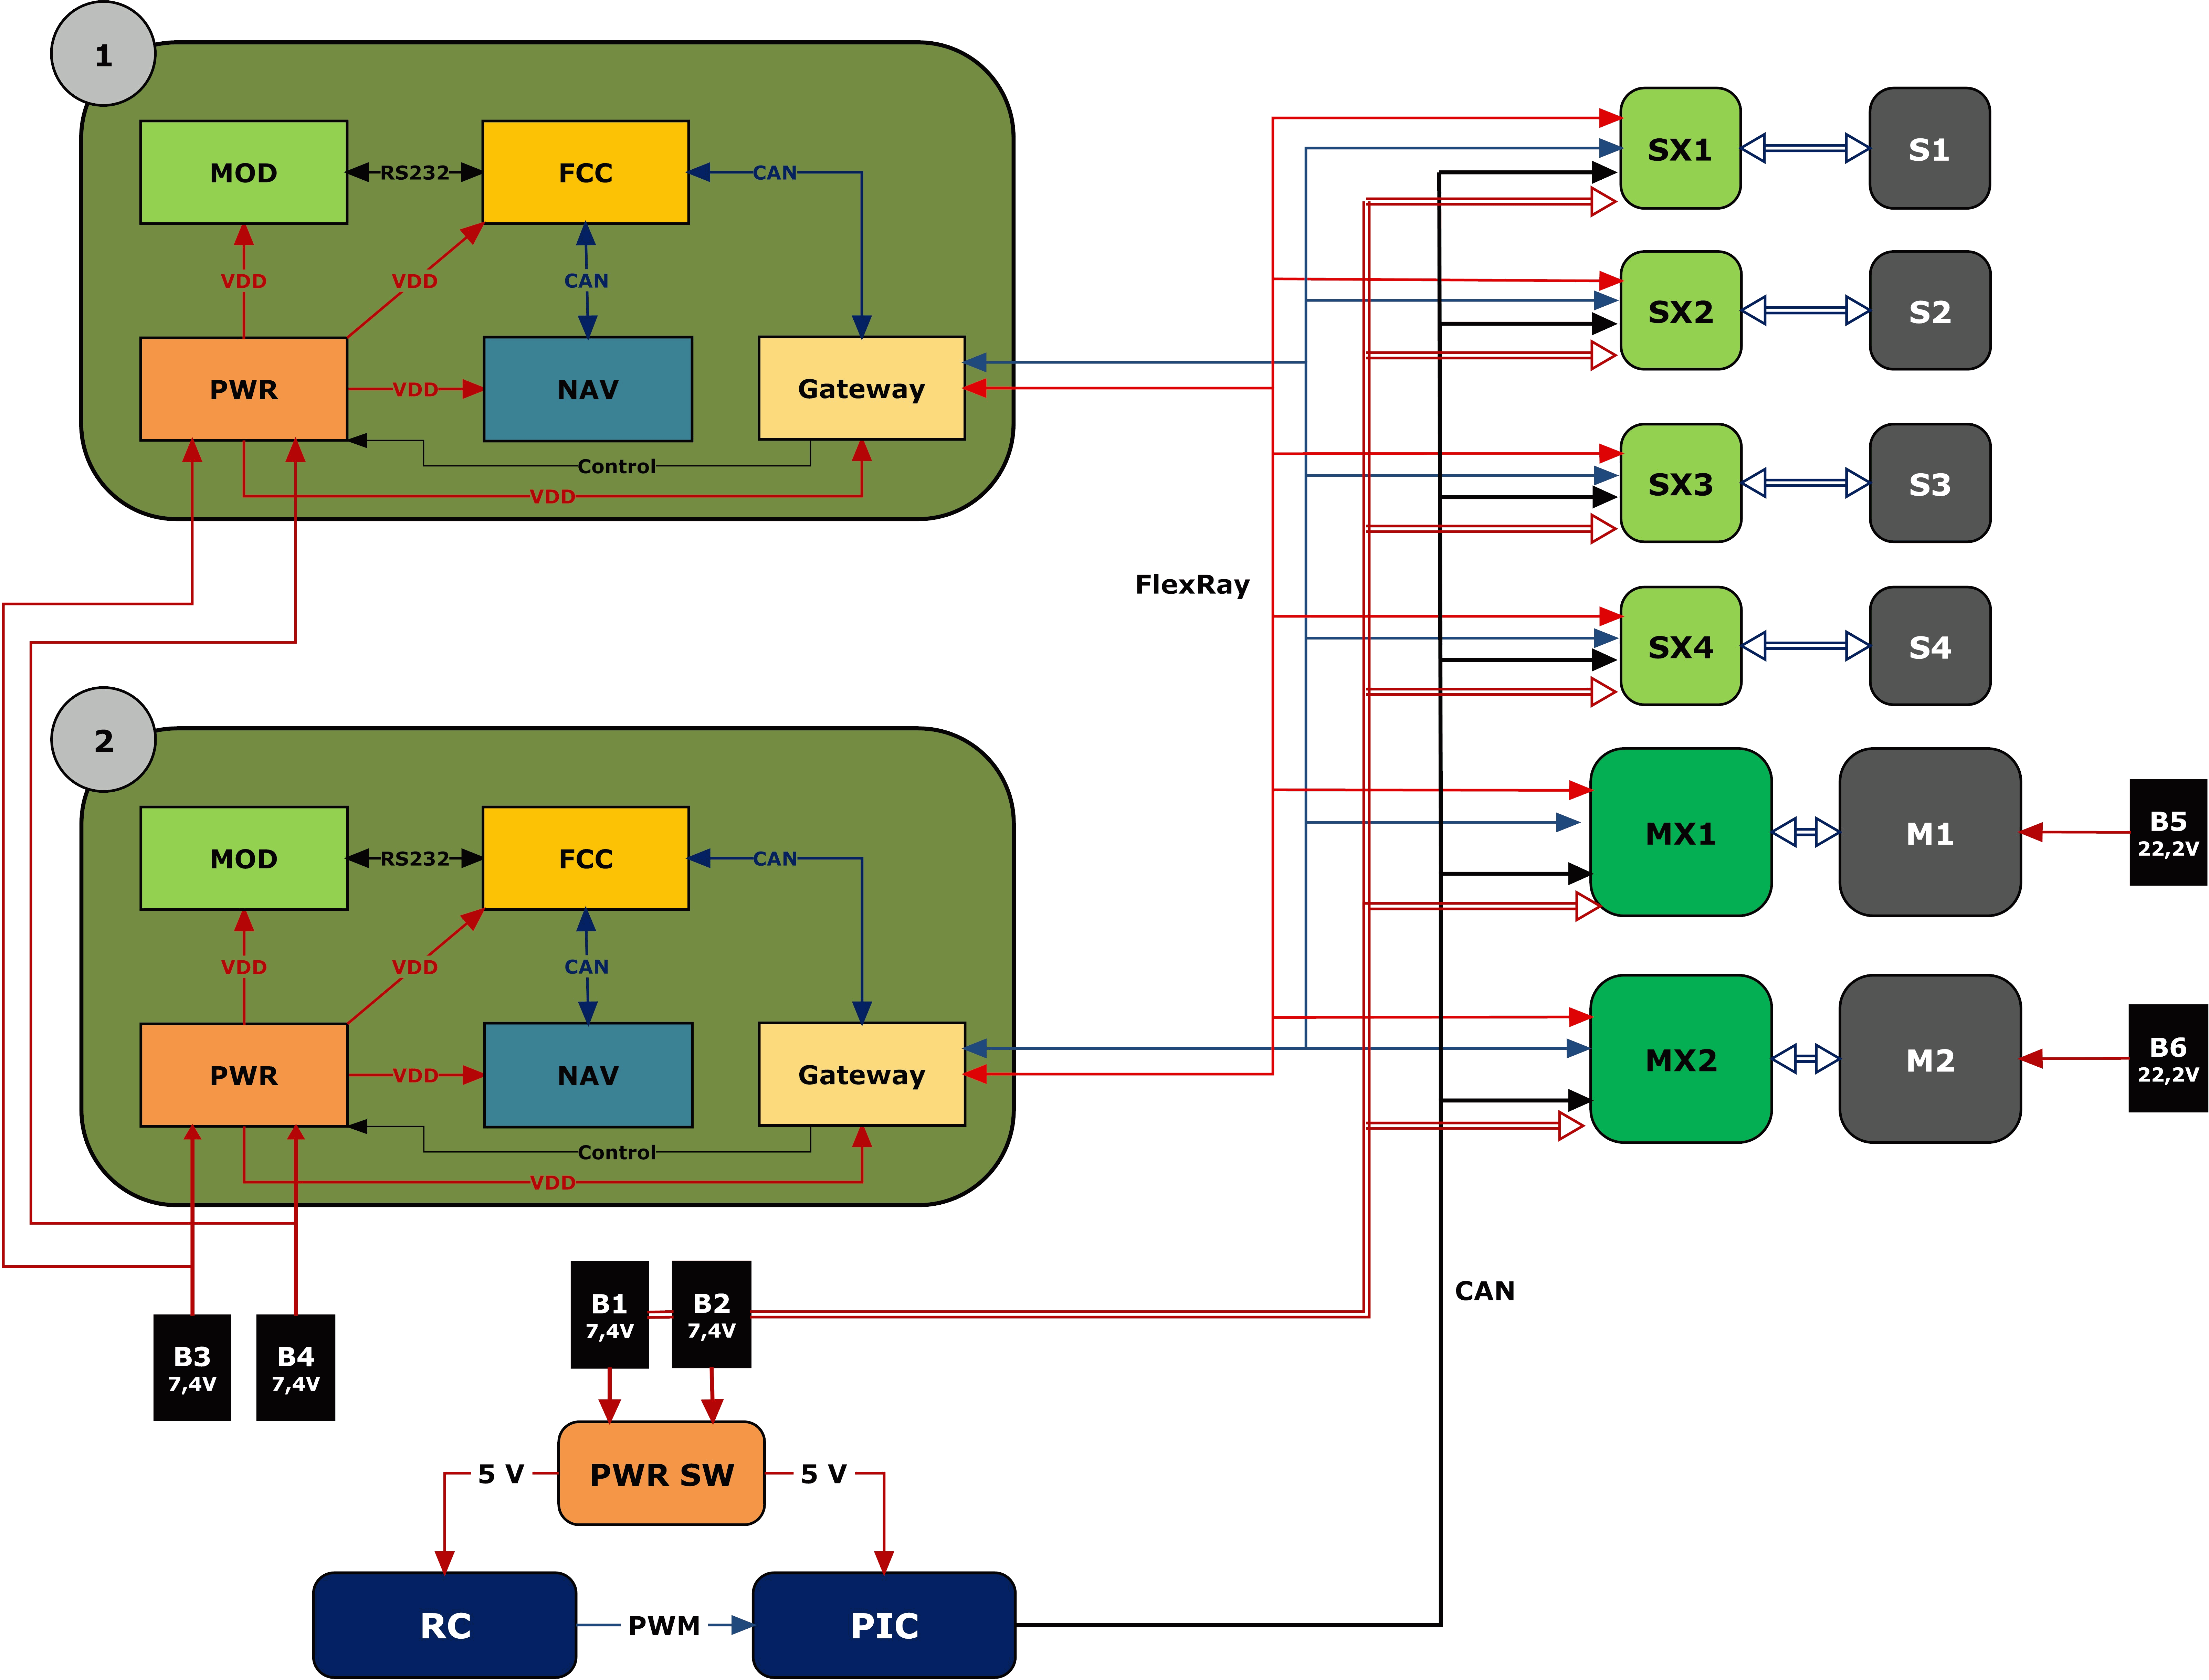
\includegraphics{sys.png}}
	\caption{}
	\label{fig:sys}
\end{figure}

Látható, hogy központi számítógép kett\H{o}zött, párhuzamosan m\H{u}ködnek, irányítják a servo motorokat. A szenzorokból érkez\H{o} jelek egy Gateway-en keresztül az FCC-be jutnak, ahol a feldolgozás utána a szabályozó algoritmusok kiadják a megfelel\H{o} utasítást a kormányszerveknek. Ilyen utasítás lehet pl, a cs\H{u}r\H{o}lapok adott fokban történ\H{o} elmozdítása, motor fordulatszámának változtatása. A motorok, úgy mint a központi egység, külön tápellátást kapnak, ezzel is csökkentve a végzetes meghibásodás esélyét. Jelen esetben egyik legfontosabb elem a kommunikációért felel\H{o}s modem, mely soros porton keresztül kapcsolódik az FCC-hez. A vev\H{o} oldalon hasonló modem, szintén soros porton küldi a földi állomásnak a vett jelet, a köztük lév\H{o} vezeték nélküli kommunikáció saját szabványa a cégnek. A választás XBee-PRO 868 típusú modemre esett, mely alacsony fogyasztása és nagy hatótávolsága miatt ideális egy ilyen környezetbe.


\begin{figure}[H]
	\centering
	\resizebox{7cm}{!}{
		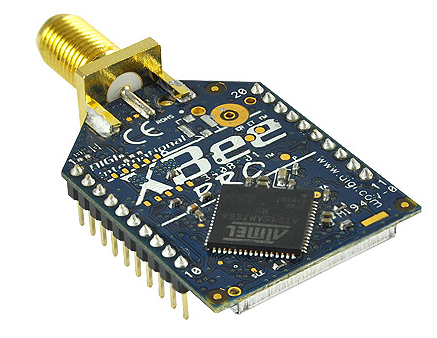
\includegraphics{xbee.png}}
	\caption{}
	\label{fig:xbee}
\end{figure}





\section{Saját implementáció}

\subsection{RS232}
A modemb\H{o}l érkez\H{o} adatokat soros porton keresztül fogadja a program, a tesztkörnyezet felállításához HIL adatok szolgáltak. A küldött log fájlokat egy programmal beolvasom és egy \cite{bib:null}null-modem segítségével sorosporton keresztül küldöm a megfelel\H{o} portra. 

\begin{figure}[H]
	\centering
	\resizebox{10cm}{!}{
		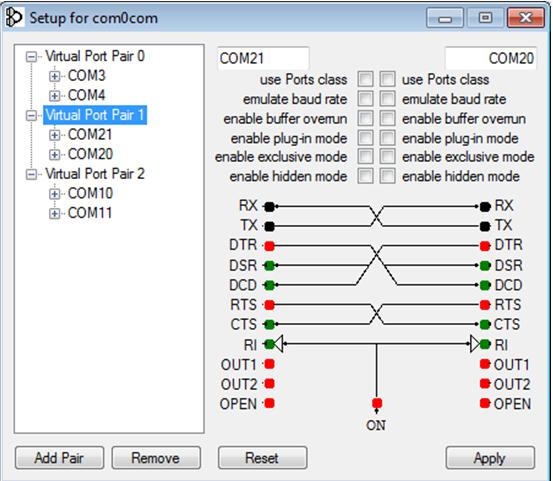
\includegraphics{comnull.png}}
	\caption{}
	\label{fig:comnull}
\end{figure}

Beállítottam 2 párt, COM20-COM21 és COM10-COM11 közt, a pároson küldöm, páratlanon fogadom az üzeneteket. 

\begin{figure}[H]
	\centering
	\resizebox{10cm}{!}{
		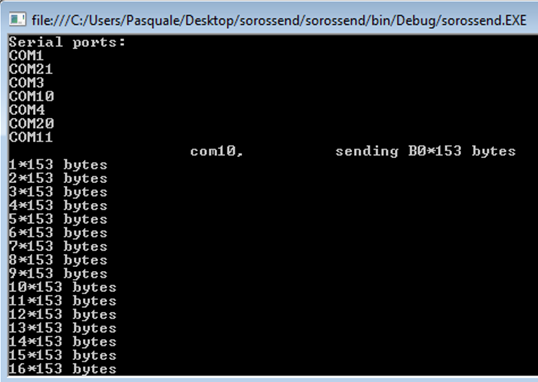
\includegraphics{sorossend.png}}
	\caption{}
	\label{fig:sorossend}
\end{figure}

153 bájtos egy csomag, melyet egy UUT  3 bájtos fejléc és egy 2 bájtos checksum zár. A checksum a hasznos bájtok 16 bitre csonkolt összege. Minden fogadott csomagnál, a feldolgozás el\H{o}tt kiszámolom az összeget és ellen\H{o}rzöm, az egyezést, a rossz csomagok egyel\H{o}re eldobásra kerülnek.

\begin{figure}[H]
	\centering
	\resizebox{10cm}{!}{
		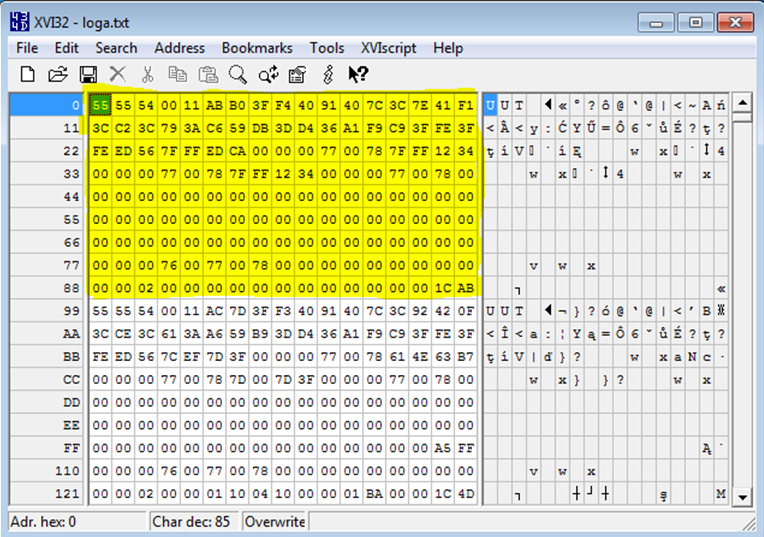
\includegraphics{xvi.png}}
	\caption{}
	\label{fig:xvi}
\end{figure}

Fogadó oldalon a két sorosport aszinkron ír 1-1 byte tömböt, melyb\H{o}l egy dekódoló függvénnyel nyerjük ki a sebesség, pozíció, irány, stb. adatokat.

\begin{verbatim}
public double[] Decode(byte[] array)
\end{verbatim}

Ebben a függvényben ellen\H{o}rzöm, a checksum-ot, illetve a kezd\H{o} UUT bájt hármast.
Mivel bájtosával lehet feldolgozni az adatokat, így pl. a 4 bájtos id\H{o}bélyeget 4 db egymás után jöv\H{o} bájtból kell összerakni:

\begin{verbatim}
uint ido = (uint)array[3]<<24 | (uint)array[4]<<16 |
(uint)array[5]<<8 | (uint)array[6];
\end{verbatim}

Ugyanígy folytatódik az adatok feldolgozása, az el\H{o}re megadott protokoll szerint.

\begin{center}
    \begin{tabular}{| l | l | l | l |l |}
    \hline
    bájt index & leírás & típus & skálázás & offset \\ \hline
    1 & start & char(fix 'U') &   &    \\ \hline
		2 & start & char(fix 'U') &   &    \\ \hline
		3 & start & char(fix 'T') &   &    \\ \hline
		4 & id\H{o} 1/4 & unsigned int & 10000 & 0  \\ \hline
		5 & id\H{o} 2/4 &   &   &    \\ \hline
		6 & id\H{o} 3/4 &   &   &    \\ \hline
		7 & id\H{o} 4/4 &   &   &    \\ \hline
		\dots &  &  &   &    \\ \hline
		26 & északi irány 1/2 & unsigned short & 0x7FFF/400 &  200 \\ \hline
		28 & keleti irány 1/2 & unsigned short & 0x7FFF/400 &  200 \\ \hline
		30 & lefelé irány 1/2 & unsigned short & 0x7FFF/400 &  200 \\ \hline
		\dots &   &   &   &    \\ \hline
		
    \hline
    \end{tabular}
\end{center}


Mivel a változások Hamming-távolsága\footnote{Bináris számok XOR képzésével kapott 1-esek száma} kicsi lenne, az eredeti számábrázoláson, így skálázással és offset képzéssel megnöveljük. A sebesség adatoknál a visszakódolás:\\
$eredeti  = (nyers adat/skalazas) - offset$ képlettel oldható meg. 

\subsection{Sebesség}
A sebesség NED\footnote{Nort East Down, Local Tangent Pane, helyi koordináta rendszer} koordinátarendszerben van megadva, mely a repül\H{o} középpontjából indul. Mivel kis magasságban repül a repül\H{o}, így síknak közelíthetjük  a Föld felületét, ez számítások szempontjából el\H{o}nyös, mivel könnyebb vele dolgozni.
A sebesség számítási módja: $ \sqrt[2]{(V_E)^2 + (V_N)^2}$ \\
Emelkedés: $ -V_D$
\begin{figure}[H]
	\centering
	\resizebox{8cm}{!}{
		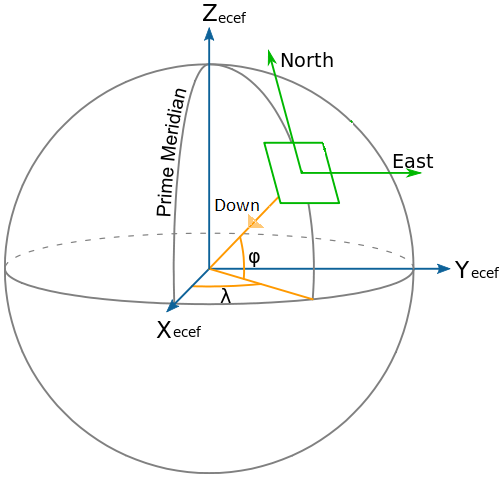
\includegraphics{ned.png}}
	\caption{Koordináta rendszer}
	\label{fig:ned}
\end{figure}

\subsection{Repülési irány}
A fedélzeten lév\H{o} mágneses irányt\H{u} irányszöge és a GPS-b\H{o}l érkez\H{o} sebesség vektor a szél következtében eltér\H{o} lehet. E kett\H{o} adatból kés\H{o}bbiekben a szél iránya is meghatározható.
Az valós irány kiszámításához a 4 negyedsíkot külön kellett választani:
\begin{verbatim}
					if (Ecomp > 0 && Ncomp > 0)
					{
						heading = Math.Atan(Ecomp * Ncomp);
					}
					else if (Ecomp > 0 && Ncomp < 0)
					{
						heading = Math.Atan(Ecomp * Math.Abs(Ncomp)) + 90;
					}
					else if (Ecomp < 0 && Ncomp < 0)
					{
						heading = Math.Atan(Math.Abs(Ecomp) * Math.Abs(Ncomp)) + 180;
					}
					else if (Ecomp < 0 && Ncomp > 0)
					{
						heading = Math.Atan(Math.Abs(Ecomp) * Ncomp) + 270;
					}

\end{verbatim}

\subsection{GUI}
A grafikus felület kialakítása során figyelembe kell venni, hogy els\H{o} ránézésre a legfontosabb adatok látszódjanak. Kett\H{o} fül közül az els\H{o} oldalon a legfontosabb m\H{u}szerek találhatóak, jobb oldalon egy Google Maps térkép. A térkép egy lokális cache-b\H{o}l tölti be az el\H{o}re letöltött térképszelvényeket, így a terepen lehet\H{o}ség van offline módon is használni ezt a funkciót.

\begin{figure}[H]
	\centering
	\resizebox{10cm}{!}{
		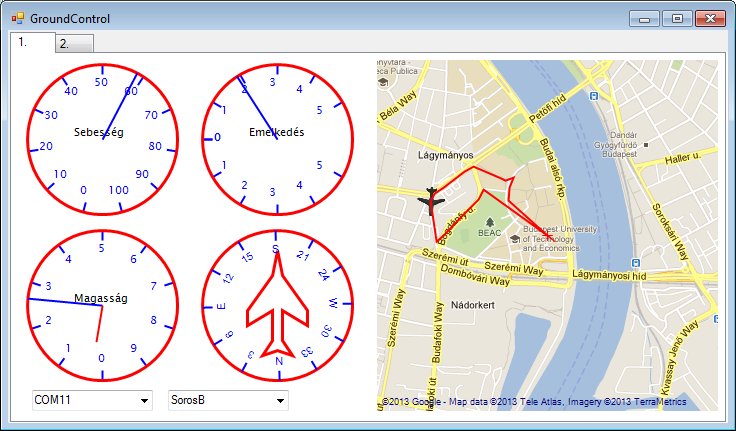
\includegraphics{gui.png}}
	\caption{}
	\label{fig:gui}
\end{figure}

A második fülön telemetria adatokat figyelhetünk meg, mely jelenleg tesztelés céljából az összes küldött adatot megjeleníti.

\begin{figure}[H]
	\centering
	\resizebox{10cm}{!}{
		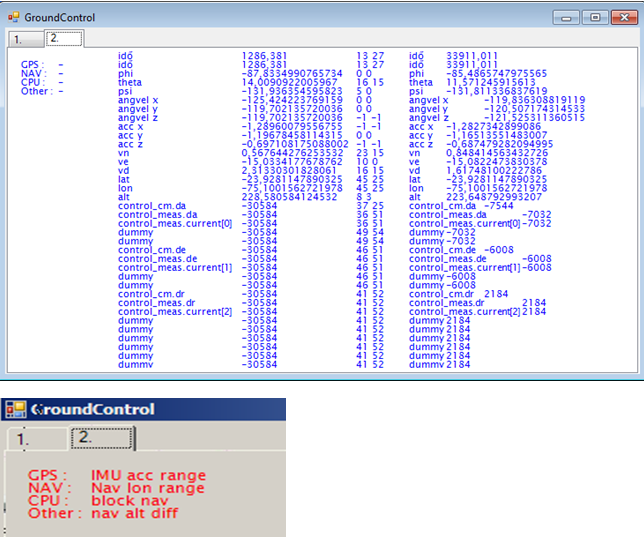
\includegraphics{gui2.png}}
	\caption{}
	\label{fig:gui2}
\end{figure}

Bal oldalt, a fedélzeti hibát, hibakódja alapján jelzi ki. Els\H{o} oszlop a küldött telemetria adat neve található, mellette az adat értéke, következ\H{o} az A és a B adat hibaszámlálója. Jelenleg a szimuláció okozta hibák miatt nagy az eltérés az adatok között, így a kés\H{o}bbi finomhangolás után, a magasságban (,,alt’’) látható 5 m különbségre folyamatosan növekedne a számlálója. Ha egy küszöbérteket elér, akkor piros színnel, illetve felt\H{u}n\H{o} hibaüzenettel jelezzük a problémát.


\section{Hibadetektálás}

\subsection{Beragadás} Ez a fajta hiba, valamelyik egység meghibásodását jelzi.  Egy $\epsilon$ tartományon belül változik a jel egy hibaszámlálót növelünk 5 egységgel.

\begin{figure}[H]
	\centering
	\resizebox{10cm}{!}{
		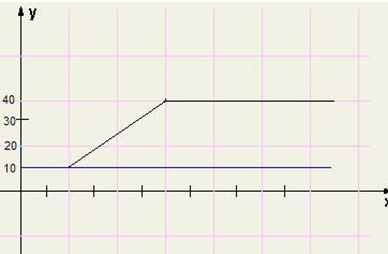
\includegraphics{hiba1.png}}
	\caption{}
	\label{fig:hib1}
\end{figure}


\subsection{Nagy változás} Az eddigi minta lapján, ha 10\%-nál nagyobb eltérés található, a számlálója növekszik 2 egységgel. Piros pont jelzi ~\ref{fig:hib2} .ábrán, a változás mértékét.

\begin{figure}[H]
	\centering
	\resizebox{10cm}{!}{
		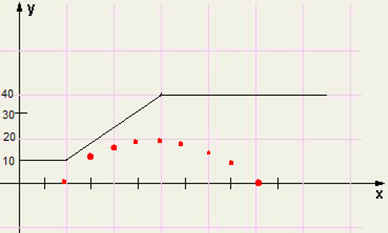
\includegraphics{hiba2.png}}
	\caption{}
	\label{fig:hib2}
\end{figure}


\subsection{Nagy eltérés a két adat között} Ha a két adatsorozat között egy $\epsilon_2$ különbség mutatkozik, növeljük a számlálót, amúgy csökkentjük. Így a gyors változásból adódó hibadetektálást kompenzáljuk, ha A és B együtt változik.


\begin{figure}[H]
	\centering
	\resizebox{10cm}{!}{
		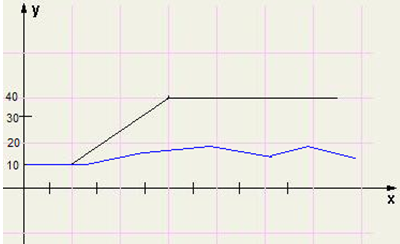
\includegraphics{hiba3.png}}
	\caption{}
	\label{fig:hib3}
\end{figure}

\section{.NET vs UNIX}
A .NET alapvet\H{o}en Microsoft technológia, de pl. a C\# könny\H{u} fejleszthet\H{o}sége miatt lehet\H{o}ségünk van .NET-ben írt alaklamazások UNIX rendszeren való futtatására is.
Erre szolgál segítségünkre a \cite{bib:mono}Mono több platformos rendszer, mely megvalósítja a .NET keretrendszert és a CLR\footnote{Common Language Runtime}-t, így ha úgy adódik, hogy a Ground Control állomás platformot vált, az eddig megírt program ,,portolható'' másik operációs rendszerre.


Tesztelhetjük is programjainkat, hogy kompatibilis-e a Monoval:
\begin{figure}[H]
	\centering
	\resizebox{10cm}{!}{
		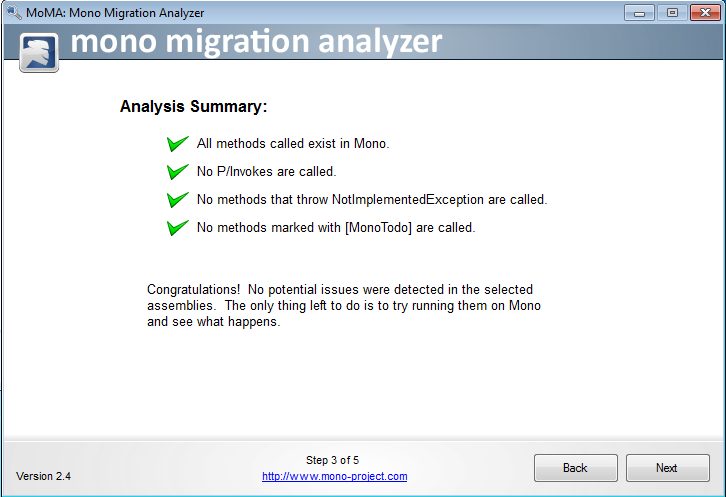
\includegraphics{mono1.png}}
	\caption{Mono}
	\label{fig:mono}
\end{figure}


\begin{thebibliography}{9}


\bibitem{bib:uav}
http://en.wikipedia.org/wiki/Unmanned\_aerial\_vehicle, 2013.~május~4, 10:00

\bibitem{bib:sperry}
http://en.wikipedia.org/wiki/Hewitt-Sperry\_Automatic\_Airplane, 2013.~május~4, 10:00

\bibitem{bib:ucav}
http://en.wikipedia.org/wiki/Unmanned\_combat\_air\_vehicle, 2013.~május~4, 10:00

\bibitem{bib:komp}
http://www.defenseindustrydaily.com/uav-ground-control-solutions-06175/, 2013.~május~4, 10:00



\bibitem{bib:mit}
http://api.ning.com/files/ga5AVWy8xTu8cx9rHdzJ73Epc*dzb0uy*UPe0O8wFxogMF6WNRW8StK3x-xzkG2iBk16kNFpYTZe80NgM8kbXOiyxrEwUXIt/GroundControlStation.pdf, 2013.~március~19., 15:00

\bibitem{bib:rodan}
http://www.rodiangroup.com/uav-ground-control-station.html, 2013.~március~19., 15:00

\bibitem{bib:hk}
https://code.google.com/p/ardupilot-mega/wiki/HappyKillmore, 2013.~március~19., 16:00

\bibitem{bib:viking}

http://www.vikingaero.com/uav\_ground\_control\_station.html, 2013.~március~19., 16:00

\bibitem{bib:mono}
http://www.mono-project.com, 2013.~március~19., 17:00

\bibitem{bib:serial}
http://msdn.microsoft.com/en-us/library/system.io.ports.serialport.aspx, 2013.~március~20, 10:00





\bibitem{bib:null}
http://com0com.sourceforge.net/, 2013.~május~4, 10:00


\end{thebibliography}

\end{document}
